% !TeX spellcheck = cs_CZ
\begin{example}\label{fyz:fey_exam010}
  Závaží o hmotnosti \(m = \SI{50}{\kg}\) je zavěšeno uprostřed drátu \texttt{ABC}, jak je 
  vidět na obrázku; \(AC = \SI{5}{\m}\), \(AB = 5\sqrt{2}\si{\m}\). Určete napěťové síly drátu 
  \(T_1\), a \(T_2\).
      
  {\centering
   \captionsetup{type=figure}
   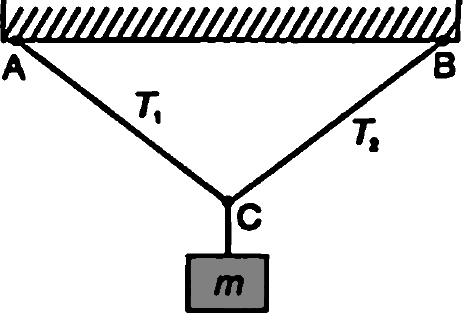
\includegraphics[width=0.4\linewidth]{fyz_fig055.png}
   \captionof{figure}{K příkladu \ref{fyz:fey_exam010} \cite[s.~60]{Feynman01}
   \label{fyz:fig055}}
  \par}
  
  Všimněme si, že \(AC\) a \(BC\) svírají pravý úhel a že napěťové síty \(T_1 = T_2 = T\) jsou 
  stejné. Úlohu bychom mohli řešit prostým rozkladem tíhy závaží \(m\) do složek. Máme-li 
  použít princip virtuálních posunutí, můžeme si třeba představit, že část drátu \(AC\) malinko 
  popustíme, takže se prodlouží o \(\Delta l\). Napěťová síla přitom vykoná virtuální práci 
  \(\Delta W = T\Delta l\); síla na úseku drátu \(BC\) zůstává k malému posunutí kolmá, takže 
  práci nekoná. Vykonaná práce musí být rovna změně potenciální energie závaží \(mg\Delta 
  l/\sqrt{2}\). Odtud 
  \begin{equation*}
     T = \frac{mg}{\sqrt{2}}=\SI{347}{\newton}.
  \end{equation*}
\end{example}